%========================================
% PREAMBOLO
%========================================

% === Impostazione del documento ==========================
\documentclass[12pt,a4paper,twoside,english,hidelinks]{book}
\pagenumbering{arabic}
\usepackage{setspace}
\onehalfspace

% === Regolazione dei margini =============================
\addtolength{\oddsidemargin}{30pt}
\addtolength{\evensidemargin}{-30pt}
\usepackage{fancyhdr}
\usepackage{multirow}
\usepackage{multicol}
\usepackage[section]{placeins}

% === Impostazione dei font ===============================
\usepackage[T1]{fontenc}
\usepackage[utf8]{inputenc}
\usepackage[english]{babel}
\usepackage{ae}
\usepackage{relsize}
\usepackage{csquotes}
\usepackage{amsmath}
\usepackage{amsfonts}
\usepackage{mathdots}
\usepackage{mathtools}
\usepackage[colorlinks=true]{hyperref}
\hypersetup{
	bookmarksnumbered=true,
	linkcolor=black,
	citecolor=black,
	%pagecolor=black,
	urlcolor=black,
}
\usepackage{verbatim}
\usepackage{alltt}
\DeclareMathOperator{\sgn}{sgn}
\DeclarePairedDelimiter{\abs}{\lvert}{\rvert}
\DeclarePairedDelimiter{\norma}{\lVert}{\rVert}

% === Integrazione delle figure ===========================
\usepackage{graphicx}
\graphicspath{{./imgs/}}
\renewcommand{\figurename}{Fig.}
\usepackage{subfig}
\usepackage[font=small,labelfont=bf]{caption}
\usepackage{wrapfig}

% === Per le tabelle ====================================
\usepackage{tabularx}
\usepackage{array}
\usepackage{color}
\usepackage{colortbl}
\usepackage{pgfplotstable}
\usepackage{makecell}
\usepackage{booktabs}

% === Per la bibliografia multicolonna =======================
\usepackage{etoolbox}
\patchcmd{\thebibliography}{\list}{\begin{multicols}{2}\smaller\list}{}{}
\appto{\endthebibliography}{\end{multicols}}
%==Per le figure latex===================================
%Package e librerie per TikZ e PGF,le librerie non sono tutte necessarie a questo documento LATEX.
\usepackage{tikz,fp,ifthen,fullpage,pgfmath,xparse,tikz-dimline}
\usetikzlibrary{decorations,backgrounds,fit,calc,through}
\usetikzlibrary{arrows,shadows,shapes}
\usetikzlibrary{fadings,patterns,mindmap}
\usepackage{pgfplots}
\pgfplotsset{compat=1.13}

% === Per gli algoritmi ===================================
\usepackage{algorithmicx}
\usepackage[ruled]{algorithm}
\usepackage{algpseudocode}
\usepackage{xcolor}
\usepackage{listings}

% === APDL STYLE LANGUAGE ==================================
\newcommand{\listingautocaption}[2][]{%
\lstinputlisting[caption={\texttt{\detokenize{#2}}},#1]{#2}%
}
%colori per il linguaggio
\definecolor{darkpastelpurple}{rgb}{0.59,0.44,0.84}
\definecolor{halfgray}{gray}{0.55}
\definecolor{arylideyellow}{rgb}{0.91,0.84,0.42}
\definecolor{cadmiumgreen}{rgb}{0.0,0.42,0.24}
\definecolor{ceruleanblue}{rgb}{0.16,0.32,0.75}
\definecolor{cinnamon}{rgb}{0.82,0.41,0.12}
\definecolor{darkslateblue}{rgb}{0.28,0.24,0.55}
\lstdefinelanguage{apdl-modified}
{
	alsoletter=/*\%,
	morekeywords={/clear,/filnam,/title,/unit,/inquire,/rep,/ang,/eshape,/replot,/view,/exit,/replo,/plopts,/triad,/efacet,/rgb,/show,/gile,/eof,/solve,/output,/out,/device
	},
	morekeywords={*afun,*dim,*vget,*do,*enddo,*cfopen,*vwrite,*cfclos,*set,
	 			*get,*use,*abbr,*msg,*if,*else,*endif,*abset,*abcheck,*abfini},
	morekeywords={start,new,finish,si,antype,static,set,deg,num,max,min,dim,
				count,line,llist,lplot,pngr,fast,leng,arotat,allsel,lsel,s,a,r,u ,
	 			none,acel,pstres,dl,mxpand,modopt,lumpm,d,save,eplot,modal,plnsol,
	 			sum,eqv,loc,eq,then,k,n,e,et,mp,ex,nuxy,dens,latt,lmesh,lesise,
	 			sectype,secoffset,secdata,keyopt,mshkey,ksel,nesl,lsel,kp,
				node,line,sect,mshape,amesh,aesize,secnum,type,real,
				mat,nslk,nsel,cyl4,wpcsys,csys,wpoffs,wprota,cerig,
				secjoint,joint,revo,esel,cm,elem,ui,x,y,z,
				lesize,solve,pldisp,sequ,l,mode,freq,coriolis,qrdamp,
				wpstyle,fill,secd,nsll,clocal,outpr,elform,elprep,nplot,psolve,
				secp,ncomp,cdsys,rect,csolid,etyp},
	otherkeywords={/angle},
	keywords=[2]{beam188,beam189,shell181,mpc184,combin14,mass21},
	keywords=[3]{/prep7,/solu,/post1,/post26},
	keywords=[5]{ARRAY,TABLE},
	keywords=[4]{
				',
				-,
				",
				\%,
				(,
				),
				,,
				.,
				:,
				;,
				?,
				^,
				−,
				+,
				<,
				=,
				>,
				e,
	},
	%define string
	morestring=[b]\%,
	morestring=[b]',%
	morestring=[b]",%
	morestring=[s]{r'}{'},% `raw' strings
	morestring=[s]{r"}{"},% `raw' strings
	morestring=[s][\color{red}\bfseries]{\%}{\%},% `raw' strings
	sensitive=false,% keywords are not case-sensitive
	%define comment
	morecomment=[l]{!},
	morecomment=[l]{/COM},
}
\lstset{
	%Frame style
	frame=single,
	rulecolor=\color{black},
	%number style
	numbers=left,
	numberstyle=\tiny\color{halfgray},
	%space and special character
	showspaces=false,
	showstringspaces=false,
	showstringspaces=false,
	breaklines=true,
	%input path
	inputpath={{./listing/}},
	extendedchars=true,
	literate=
	{á}{{\'a}}1 {é}{{\'e}}1 {í}{{\'i}}1 {ó}{{\'o}}1 {ú}{{\'u}}1
	{Á}{{\'A}}1 {É}{{\'E}}1 {Í}{{\'I}}1 {Ó}{{\'O}}1 {Ú}{{\'U}}1
	{à}{{\`a}}1 {è}{{\`e}}1 {ì}{{\`i}}1 {ò}{{\`o}}1 {ù}{{\`u}}1
	{À}{{\`A}}1 {È}{{\'E}}1 {Ì}{{\`I}}1 {Ò}{{\`O}}1 {Ù}{{\`U}}1
	{ä}{{\"a}}1 {ë}{{\"e}}1 {ï}{{\"i}}1 {ö}{{\"o}}1 {ü}{{\"u}}1
	{Ä}{{\"A}}1 {Ë}{{\"E}}1 {Ï}{{\"I}}1 {Ö}{{\"O}}1 {Ü}{{\"U}}1
	{â}{{\^a}}1 {ê}{{\^e}}1 {î}{{\^i}}1 {ô}{{\^o}}1 {û}{{\^u}}1
	{Â}{{\^A}}1 {Ê}{{\^E}}1 {Î}{{\^I}}1 {Ô}{{\^O}}1 {Û}{{\^U}}1
	{œ}{{\oe}}1 {Œ}{{\OE}}1 {æ}{{\ae}}1 {Æ}{{\AE}}1 {ß}{{\ss}}1
	{ç}{{\c c}}1 {Ç}{{\c C}}1 {ø}{{\o}}1 {å}{{\r a}}1 {Å}{{\r A}}1
	{€}{{\EUR}}1 {£}{{\pounds}}1 {θ}{{$\theta$}}1 {Φ}{{$\Phi$}}1,
	% defie style
	basicstyle=\scriptsize\ttfamily,
	% style of keyword
	% keyword
	keywordstyle=\color{ceruleanblue}\bfseries\ttfamily,
	%type elements
	keywordstyle=[2]\color{darkslateblue},
	% section
	keywordstyle=[3]\color{cinnamon},
	keywordstyle=[4]\color{black},
	keywordstyle=[5]\color{arylideyellow},
	% style of comments
	commentstyle=\color{cadmiumgreen}\ttfamily,
	% style of string
	stringstyle=\color{darkpastelpurple}\ttfamily,
}

%========================================
% TESTO DELLA TESI
%========================================

\begin{document}
	% === Frontespizio ====================================
	\pagestyle{empty}
	%%%%%%%%%%%%%%%%%%%%%%%%%%%%%%%%%%%%%%%%%%%%%%%%%%%%%%%%%%%
% Frontespizio
%%%%%%%%%%%%%%%%%%%%%%%%%%%%%%%%%%%%%%%%%%%%%%%%%%%%%%%%%%%
\begin{titlepage}
 \begin{center}
 
\includegraphics[width=3.5cm]{unitn.jpg}\\
 \vspace{1em}
 {\Large \textsc{Università degli studi di Trento}}\\
 \vspace{1em}
 {\Large \textsc{Dipartimento di Ingegneria Industriale}}\\
 \vspace{4em}
 {\normalsize Relazione}\\
 \vspace{1em}
 {\Large \textsc{Mechanical Vibrations}}\\
 \vspace{4em}
 {\LARGE\textbf{
 	System identification of a 3 DOF system
 }}\\
 \end{center}

\vskip 2.0cm
 \begin{center}
 \begin{tabular}{c c c c c c c c}
 Relatore & & & & & & & Candidato \\[0.2cm]
 \large{Prof. Daniele Bortoluzzi} & & & & & & & \large{Francesco Aregntieri}\\[0.4cm]
 Correlatore & & & & & & & ID: 183892\\[0.2cm]
 \large{Dott. Egidio Labbate}& & & & & & &\\
 \end{tabular}
 \end{center}

\vskip 1.5cm
\begin{center}
{\normalsize Anno Accademico 2015/2016}
\end{center}
\end{titlepage}

\clearpage{\pagestyle{empty}\cleardoublepage}

	% === Indice =========================================
	\tableofcontents

	% === Capitoli Tesi ===================================
	\pagestyle{plain}
	%%%%%%%%%%%%%%%%%%%%%%%%%%%%%%%%%%%%%%%%%%%%%%%%%%%%%%%%%%%

\chapter{Introduzione}
\label{chap:Introduzione}

%%%%%%%%%%%%%%%%%%%%%%%%%%%%%%%%%%%%%%%%%%%%%%%%%%%%%%%%%%%

\section{Contesto applicativo}
\label{sec:intro1}

Ciao ragazzi :D questo è un template che potete utilizzare per scrivere la vostra tesi in \LaTeX (sì, il nome di questo linguaggio è tutto un programma...)

Cos'è \LaTeX ? Cercatevelo su Wikipedia\footnote{http://it.wikipedia.org/wiki/LaTeX}!

A parte gli scherzi... è un linguaggio che vi permette (in poche parole) di creare documenti accademici (e non) con uno stile molto professionale. Gran parte del lavoro sporco (creazione dei capitoli, delle sezioni, dell'indice, della bibliografia, gestione dei margini, ecc...) viene interamente gestito da \LaTeX , le poche cose da configurare sono già state impostate in questo template... (quindi in poche parole avete già tutto pronto, stronzi!)

In questo pdf è spiegato un po' come far funzionare il tutto, ovvero:
\begin{itemize}
\item Dove scaricare l'IDE e come configurarlo
\item Come scaricare il compilatore
\item Come iniziare a personalizzare questo template
\end{itemize}

Cercherò di utilizzare più elementi \LaTeX possibile nello scrivere questa guida (tabelle, elenchi puntati, footnote, immagini...) così quando andrete a leggere il codice vi imparate pure qualcosa, caproni (<3)

%%%%%%%%%%%%%%%%%%%%%%%%%%%%%%%%%%%%%%%%%%%%%%%%%%%%%%%%%%%

\section{Motivazioni e obiettivi}
\label{sec:intro2}

Il principale motivo che mi spinge a creare questo pdf è quello di risparmiarvi gran parte delle rotture che si trovano quando ci si avvicina al mondo \LaTeX... insomma mi auguro che questa guida vi permetta di avere un buon punto d'inizio.

Come già spiegato nella sezione precedente, \LaTeX offre tantissimi servizi utili ed uno stile professionale unico, cose che su altri programmi (come Microsoft Word) potete anche sognarvi.

Insomma... con \LaTeX potete presentare una tesi fatta come si deve :)

%%%%%%%%%%%%%%%%%%%%%%%%%%%%%%%%%%%%%%%%%%%%%%%%%%%%%%%%%%%

\section{Risultati raggiunti}
\label{sec:intro3}

Nella Figura \ref{fig:latexVsWord} potete ammirare quanto \LaTeX sia più figo di Microsoft Word, ooooooh...

\begin{figure}[h] %La "h" indica che la figura si posizionerà "here". Usate "t" per "top" e "b" per "bottom"
\centering %centrata
%\includegraphics[width=0.8\linewidth]{latexVsWord} %larghezza e nome del file
\caption{Oooooooh che figo \LaTeX, ooooooooh} %didascalia
\label{fig:latexVsWord} %label per il riferimento
\end{figure}

%%%%%%%%%%%%%%%%%%%%%%%%%%%%%%%%%%%%%%%%%%%%%%%%%%%%%%%%%%%

\section{Organizzazione della tesi}
\label{sec:intro4}

Vi spiego brevemente quali sono le parti di questo template:

\begin{description}
  \item[Susanna.tex] Questo è il file principale del template: contiene le impostazioni generali e la struttura della tesi. Ricordate di impostarlo come documento master ogni volta che iniziate a lavorare alla tesi (ovviamente potete rinominarlo, nabbazzi)
  \item[frontespizio.tex] Sarebbe la copertina della tesi, nonchè la prima pagina. Contiene nome dell'università, del dipartimento, nome della tesi bla bla bla... io ho scelto un argomento di Fisica molto importante <3
  \item[dedica.tex] Una pagina dove scrivete a chi dedicate la tesi (Susanna <3)
  \item[introduzione.tex] Il file che contiene questo capitolo introduttivo (vi consiglio di creare appunto un file .tex per ogni capitolo). Le 4 sezioni di questo capitolo (\nameref{sec:intro1}, \nameref{sec:intro2}, \nameref{sec:intro3} e \nameref{sec:intro4}) sono le 4 sezioni standard da inserire nell'introduzione di una tesi, quindi vi consiglio di lasciarle così
  \item[start.tex] Contiene l'unico capitolo utile di questo documento: spiega come scaricare l'occorrente e come configurare il tutto per lavorare con \LaTeX
  \item[conclusione.tex] Contiene la conclusione (YOU DON'T SAY)
  \item[bibliografia.bib] Contiene i dati relativi alle fonti che citerete nella tesi (ad esempio, ora sto citando un libro sugli algoritmi genetici \cite{5635176}, l'unico inserito nella bibliografia di questo template)
  \item[IEEEtran.bst] È lo stile della bibliografia, non lo toccate
  \item[imgs] Cartella contenente le immagini (YOU DON'T SAY AGAIN)
\end{description}


	%%%%%%%%%%%%%%%%%%%%%%%%%%%%%%%%%%%%%%%%%%%%%%%%%%%%%%%%%%%

\chapter{Come fare le cose}
\label{chap:omfglol}

In questo capitolo vediamo la roba smanettosa per iniziare a smanettare

%%%%%%%%%%%%%%%%%%%%%%%%%%%%%%%%%%%%%%%%%%%%%%%%%%%%%%%%%%%

\section{Occorrente}
\label{sec:occorrente}

Roba da scaricare e installare (Tabella \ref{tab:filesize}).

\begin{table}[h]
\centering
\caption{Tabella vergognosamente inutile}
\vspace{0.3cm}
\label{tab:filesize}
\begin{tabular}{lll}
 \hline
File & Piattaforma & Dimensioni \\\hline
\emph{TexMaker} & Windows & 46.3 MB \\
\emph{TexMaker} & Mac & 40.7 MB \\
\emph{MiKTeX} & Windows & 154.1 MB \\
\emph{MacTex} & Mac & 2.3 GB \\
Template Susanna & Multiglobale-powa & 4 MB (circa) \\\hline
\end{tabular}
\end{table}

\pagebreak

%%%%%%%%%%%%%%%%%%%%%%%%%%%%%%%%%%%%%%%%%%%%%%%%%%%%%%%%%%%

\subsection{L'IDE}
\label{sub:ide}

Allora... per prima cosa vi serve un IDE, ovvero un programma che vi funga da editor e compilatore (in realtà il compilatore si scarica a parte ma vabbè). Ce ne sono molti in giro ma io vi consiglio \emph{TexMaker}\footnote{http://www.xm1math.net/texmaker/} per due motivi:

\begin{enumerate}
\item È molto intuitivo è ben fatto
\item Esiste sia per Mac che per Windows
\end{enumerate}

Non dovreste avere problemi con il download e l'installazione (vi state per laureare porca paletta, non devo spiegarvi pure questo).

%%%%%%%%%%%%%%%%%%%%%%%%%%%%%%%%%%%%%%%%%%%%%%%%%%%%%%%%%%%

\subsection{Il compilatore}
\label{sub:compilatore}

Per quanto riguarda il compilatore il discorso è un po' più complicato. Armatevi di pazienza e scaricate \emph{MiKTeX}\footnote{http://miktex.org/download} se avete Windows oppure \emph{MacTex}\footnote{http://mirror.ctan.org/systems/mac/mactex/MacTeX.pkg} se avete un Mac (mi dispiace ma non conosco un compilatore LaTeX per Linux... se lo trovato fatemelo sapere che aggiorno la guida). Entrambi questi programmi inglobano un ambiente di sviluppo \LaTeX costituito da diversi compilatori che il nostro IDE riconoscerà automaticamente.

\textbf{P.S.} Prima che cominciate a strapparvi i capelli, sì, \emph{MacTex} occupa più di 2 GB... questo perchè comprende tutti i pacchetti necessari per \LaTeX, mentre \emph{MiKTeX} (che occupa solo 150 mb) li scarica volta per volta.

%%%%%%%%%%%%%%%%%%%%%%%%%%%%%%%%%%%%%%%%%%%%%%%%%%%%%%%%%%%

\subsection{Il template}
\label{sub:template}

Trovate il sorgente di questo template ad un link dropbox non meglio specificato\footnote{https://www.dropbox.com/sh/1f06sd7eprongvl/dKsfID1Kwc}

%%%%%%%%%%%%%%%%%%%%%%%%%%%%%%%%%%%%%%%%%%%%%%%%%%%%%%%%%%%

\section{Configurazione dell'IDE}
\label{sec:configurazioneIDE}

Oooh, ora che avete installato IDE e compilatore, lanciate l'IDE. Principalmente dovete fare tre cose una volta avviato:

\begin{enumerate}
\item Aprite il file Susanna.tex del template
\item Andate su Opzioni -> Definire il documento corrente come Master (questo serve per dire all'IDE che gli altri documenti sono inclusi in un documento master e che quindi, al momento della compilazione, non devono essere trattati come documenti separati)
\item Andate nelle preferenze dell'IDE nella sezione Compilazione Rapida e personalizzate la compilazione tramite l'assistente-wizard. Essenzialmente dovete configurarla in modo da effettuare 3 compilazioni: PdfLatex, BibTex e di nuovo PdfLatex. Oltre a queste tre compilazioni aggiungete una quarta opzione ovvero la visualizzazione pdf.
\end{enumerate}

Vi spiego meglio il punto 3... praticamente ci sono più compilatori diversi, che svolgono operazioni diverse... ma a noi interessano solo due compilatori, ovvero PdfLatex (che compila il codice \LaTeX in un documento pdf) e BibTex (che compila la bibliografia). Le compilazioni sono 3 e in quel preciso ordine perchè altrimenti la bibliografia non viene compilata bene (non chiedetemi perchè). Per evitare di dover eseguire manualmente le diverse compilazioni, \emph{TexMaker} vi dà la possibilità di utilizzare la Compilazione Rapida che esegue automaticamente queste operazioni con un click. Configuratela come vi ho spiegato e non avrete problemi.

%%%%%%%%%%%%%%%%%%%%%%%%%%%%%%%%%%%%%%%%%%%%%%%%%%%%%%%%%%%

\section{Siamo pronti}
\label{sec:pronti}

Abbiamo configurato l'IDE ed il (i) compilatore(i). Ora premendo sulla freccina della Compilazione Rapida (oppure premendo F1) potrete compilare il vostro codice \LaTeX in pdf. Fate una prova compilando il template (il pdf purtroppo, così come tutti gli scarti della compilazione, verranno generati nella stessa cartella del sorgente...).

E ora? Ora create i vostri capitoli copiando la struttura di \emph{start.tex} e di \emph{introduzione.tex} ed integrateli nel documento master :) se avete bisogno di ulteriori dettagli sulla sintassi \LaTeX vi consiglio di farvi un giro nella sezione Tex di \emph{Stack Exchange}\footnote{http://tex.stackexchange.com/}: è tipo Yahoo Answers ma focalizzato ovviamente su \LaTeX :)
	\chapter{Eurocopter AS350}
\label{ch:Eurocopter AS350}

\emph{This chapter opens with an introduction to the helicopter named Eurocopter AS350, its development over the years and some technical features. In follow deals with the study of the tail in particular \dots, where the aeroelastic problem will be neglected and as a result all the aerodynamic components will be removed from the model.}

\section{Introduction}
The \textbf{Eurocopter AS350 Écureuil} (\emph{Squirrel}) is a single-engine light helicopter originally designed and manufactured in France by Aérospatiale, now Airbus Helicopters. In North America, the AS350 is marketed as the AStar. The AS355 Ecureuil 2 is a twin-engine variant, marketed in North America as the TwinStar. The Eurocopter EC130 is a derivative of the AS350 airframe and is considered by the manufacturer to be part of the Écureuil single-engine family.
In the early 1970s, Aérospatiale decided to initiate a new development programme to produce a suitable replacement for the aging Aérospatiale Alouette II.
While the Aérospatiale Gazelle, which had been developed in the 1960s and 1970s, had been met with numerous orders by military customers, commercial sales of the type had been less than anticipated, thus the need for a new civil-orientated development was identified.
The development of the new rotorcraft, which was headed by Chief Engineer René Mouille, was focused on the production of an economic and cost-effective aerial vehicle, thus both Aérospatiale's Production and Procurement departments were heavily involved in the design process.
One such measure was the use of a rolled sheet structure, a manufacturing technique adapted from the automotive industry; another innovation was the newly developed Starflex main rotor. It was also decided that both civil and military variants of the emergent helicopter would be developed to conform with established military requirements\cite{wiki:xxx}.

\begin{minipage}{\textwidth}
  \begin{minipage}[b]{0.49\textwidth}
   	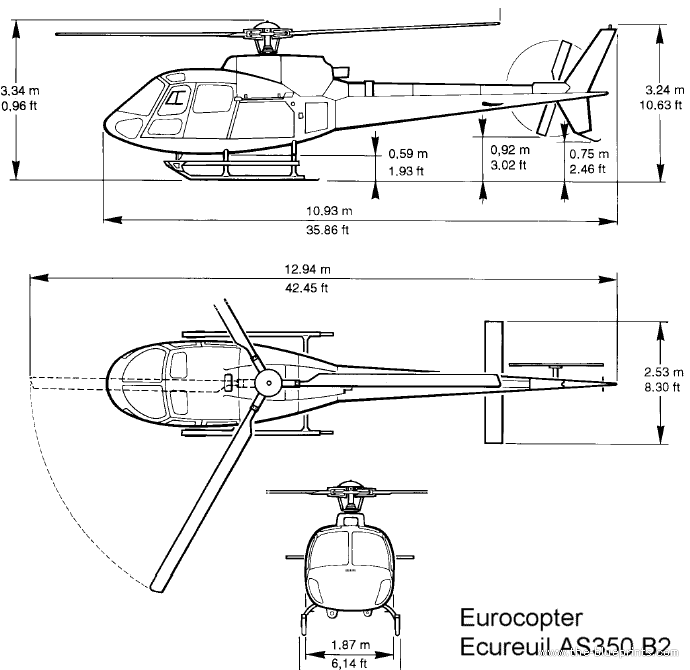
\includegraphics[width=\textwidth]{eurocopter-as350-b2}
    \captionof{figure}{AS350 blueprints\label{fig:AS350blueprints}}
  \end{minipage}
  \hfill
  \begin{minipage}[b]{0.49\textwidth}
    \centering
    \begin{tabular}{%
		>{}l%
		>{}l%
		>{\columncolor{yellow}}r}
		\multicolumn{2}{>{\columncolor{lightgray}}c}{General characteristics}\\
		Length	&	12.94 m\\
		Height	&	3.34 m\\
		Main rotor diameter& 10.69 m\\
		Empty weight		& 1220 kg\\
		Max takeoff weight & 2250 kg\\
		capability	& 2500 kg\\
		\multicolumn{2}{>{\columncolor{lightgray}}c}{Propulsion}\\
		Powerplant	&	1 x Turbine\\ 
		& Turbomeca\\& Arriel 1D1\\
		Power	&	546 kW\\
		\multicolumn{2}{>{\columncolor{lightgray}}c}{Performance}\\
		Maximum speed & 287 km/h\\
		Range	 & 476 km\\
		service ceiling 	 & 6100 m\\
    \end{tabular}
  \captionof{table}{Main characteristics AS350}\end{minipage}
\end{minipage}

\begin{figure}[t]
\centering
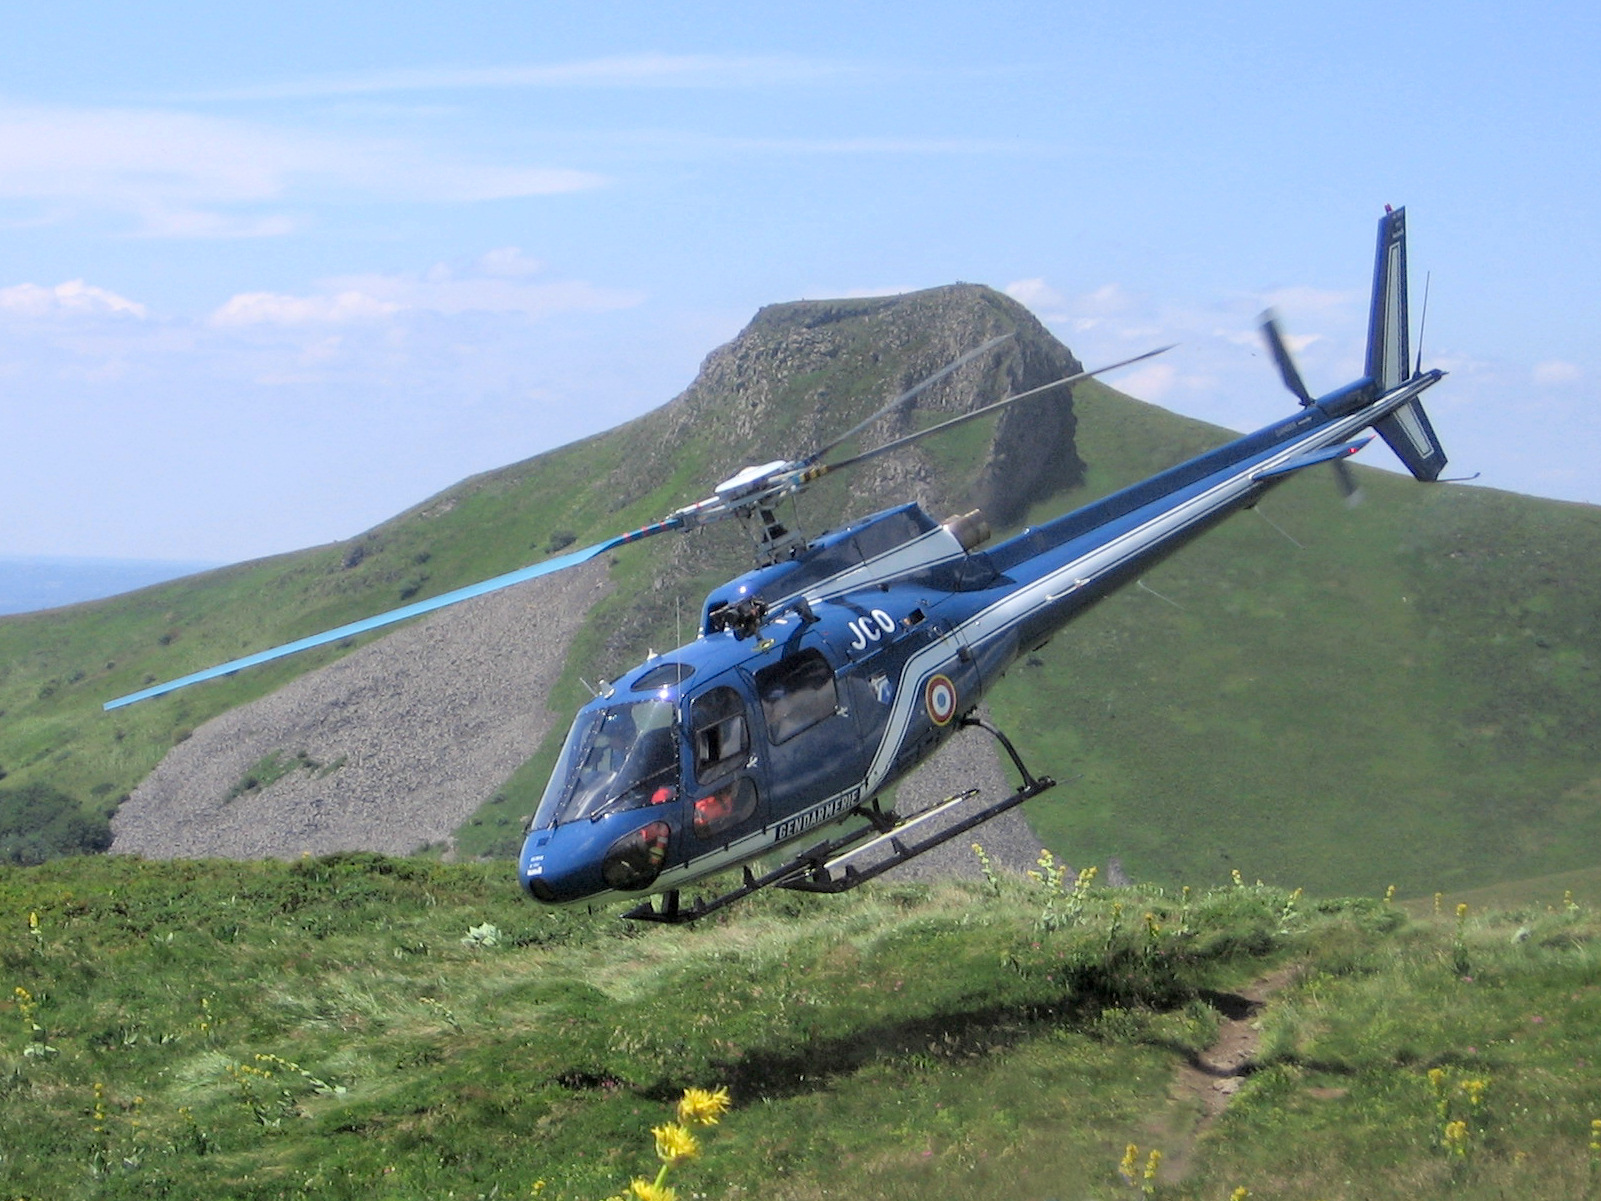
\includegraphics[width=0.80\textwidth]{Helicopter_rescue_sancy_takeoff}
\caption{Helicopter takeoff \\Di Fabien1309 - Own work}
\label{fig:AS350wiki}
\end{figure}

\section{Geometric model}

The geometric model is shared among three different configuration where was enfatizated a different approach to evalute the repsonce of structural elemtents in different condition of approximation. Infact the first case is an evalution of the simple model where considering only tail like as a cantilever beam. 
While in the second case considering also the trasmission shaft rigidly linked at the tail and the presence of a lumped mass to simulate the persence of the block of rotor in the proximity the end of tail. 
Finally consider a third model where we considering the shaft's weight is distributed along the lenght of tail like as lumped mass, we consider as before another concentrated mass to represent the block of rotor at the tail's end.
The model was obtained by the revolution of seven contiguous segments with respect to axis placed in the plane $xz$, thus obtaining a truncated cone having a radius $325\,mm$ at the base and a radius $501,mm$ for the minor base, the whole extension is $5.2\,m$.
The cone trunk was highlighted in twentyfour equal segments in order to obtain a bse for the reallization of components such as stringer, horizontal stabilizer attachment, stiffners and ribs.
The result can be seen in the figure \ref{fig:Ansys1}.

\begin{figure}[htb]
\centering
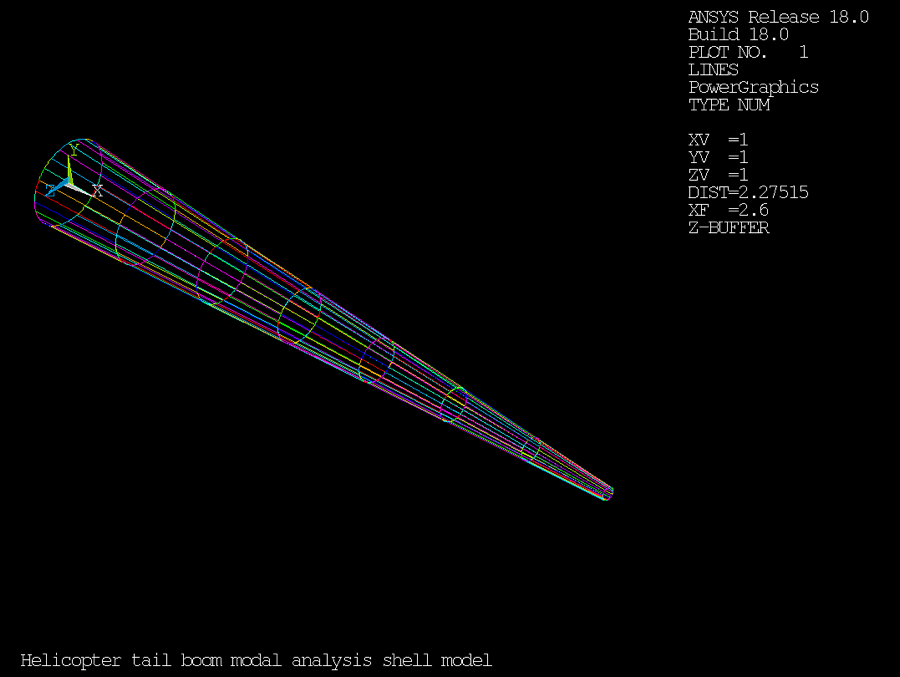
\includegraphics[width=\textwidth]{/ShellModel/Shellmodel000}
\caption{AS350 ansys model}
\label{fig:Ansys1}
\end{figure}

\section{Mesh model}
After the geometric model has been realized, the finite element model has the same types of shared elements to ensure consistency between the models, as well as the texture of the matrices used to study the different models.
\subsection{Simple model}
For structural elements such as:
\begin{itemize}
\item stringer;
\item horizontal stabilizer attachment;
\item stiffners;
\item ribs.
\end{itemize}
Type elements have been used: \textsc{beam189}, this type of element has been assigned a rectangular section and a square as shown in \ref{fig:SectionGeometry}. Specifically, the rectangular section, fig. \ref{subfig:Rectagnle}, is intended to form the stinger and longerons components, instead the square section, fig.\ref{subfig:Square}, perform the ribs.
The material used is steel with the following properties:
\begin{itemize}
\item Young's modulus, $205\,[GPa]$ 
\item Poisson's ratio, $0.29$
\item Density, $7850	\,[kg/m^3]$
\end{itemize}

\begin{figure}[htb]
\centering
\subfloat[][\emph{Rectangular}.\label{subfig:Rectagnle}]{
   \resizebox{.25\linewidth}{!}{\begin{tikzpicture}
%linee guida
%\foreach \x in {0,1,...,15}
%   \draw [help lines] (\x,0) node [below,%
%          font=\footnotesize] {$\x$} -- (\x,15);
%%\foreach \y in {0,1,...,15}
%%   \draw [help lines] (0,\y) node [left,%
%%          font=\footnotesize] {$\y$} -- (15,\y);

\node at (1,14) (a) {};
\node at (3,14) (b) {};
\node at (3,10) (c) {};
\node at (1,10) (d) {};

\draw (a) rectangle (c);
\draw[-latex] (2,12)--( 2,9.5)node[right]{\scriptsize x};
\draw[-latex] (2,12)--(3.5,12)node[above]{\scriptsize y};


% quote track
 \dimline    [color=gray,
 			  label style={above=0.1ex},
                % line style={thick},
                %extension start style={gray,thin},
                %extension end style={gray,thin},
                extension start length=0.5cm,
                extension end length=0.5cm
                ]{(1,14.5)}{(3,14.5)}{$b$};
                
\dimline    [color=gray,
                % line style={thick},
                %extension start style={gray,thin},
                %extension end style={gray,thin},
                extension start length=0.5cm,
                extension end length=0.5cm
                ]{(0.5,10)}{(0.5,14)}{$w$};
\end{tikzpicture}}} \quad
\subfloat[][\emph{Square}.\label{subfig:Square}]{
   \resizebox{.25\linewidth}{!}{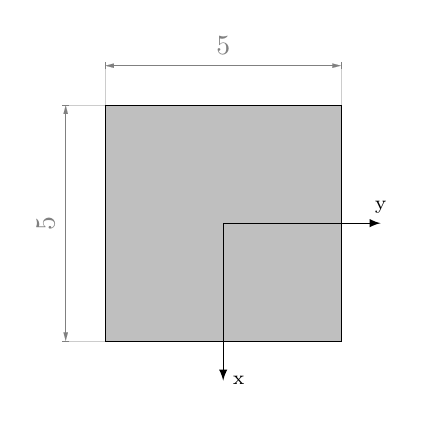
\begin{tikzpicture}
%linee guida
%\foreach \x in {0,1,...,15}
%   \draw [help lines] (\x,0) node [below,%
%          font=\footnotesize] {$\x$} -- (\x,15);
%\foreach \y in {0,1,...,15}
%   \draw [help lines] (0,\y) node [left,%
%          font=\footnotesize] {$\y$} -- (15,\y);

\node at (1,14) (a) {};
\node at (4,14) (b) {};
\node at (4,11) (c) {};
\node at (1,11) (d) {};

\draw[fill=lightgray] (a) rectangle (c);
\draw[-latex] (2.5,12.5)--( 2.5,10.5)node[right]{\scriptsize x};
\draw[-latex] (2.5,12.5)--(4.5,12.5)node[above]{\scriptsize y};


% quote track
 \dimline    [color=gray,
 			  label style={above=0.1ex},
                % line style={thick},
                %extension start style={gray,thin},
                %extension end style={gray,thin},
                extension start length=0.5cm,
                extension end length=0.5cm
                ]{(1,14.5)}{(4,14.5)}{$5$};
                
\dimline    [color=gray,
			label style={above=0.1ex},
                % line style={thick},
                %extension start style={gray,thin},
                %extension end style={gray,thin},
                extension start length=0.5cm,
                extension end length=0.5cm
                ]{(0.5,11)}{(0.5,14)}{$5$};
\end{tikzpicture}}}\\
\caption{Section for element \textsc{beam189}}
\label{fig:SectionGeometry}
\end{figure}

\noindent On the other hand, to realize the mantle covering the support structure was used type element: \textsc{shell181} with aluminum used as material with the following properties:
\begin{itemize}
\item Young's modulus: $64\,[GPa]$;
\item Poisson's ratio: $0.34$;
\item Density: $2700\,[kg/m^3]$.
\end{itemize}
Finally, you can see the full model in the figure \ref{fig:Ansys1Mesh}.

\begin{figure}[ht]
\centering
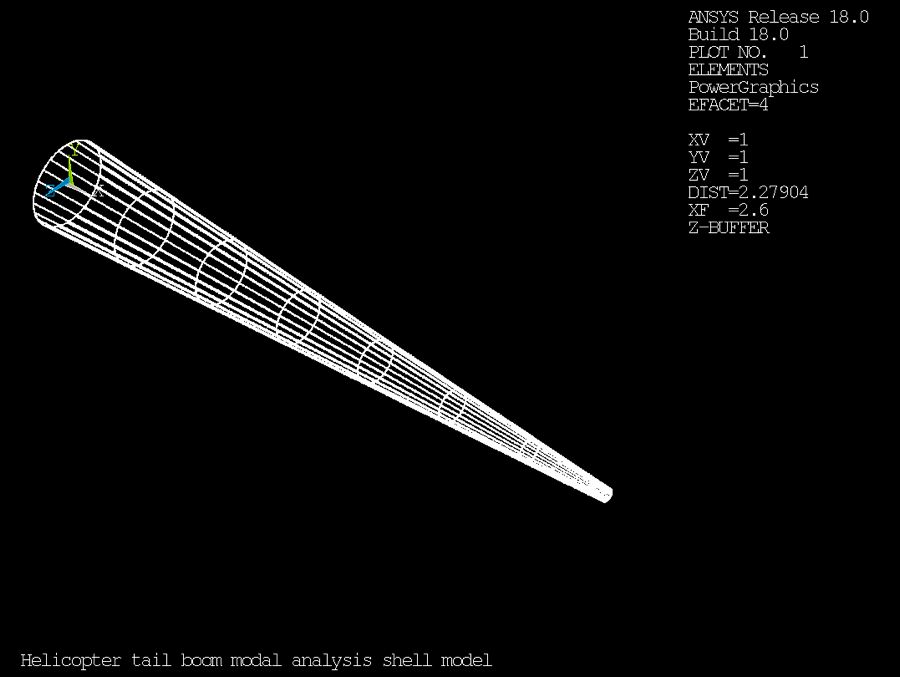
\includegraphics[width=\textwidth]{/ShellModel/Shellmodel001}
\caption{AS350 mesh model}
\label{fig:Ansys1Mesh}
\end{figure}

\subsection{Simple model with shaft}
In this case, the geometric model has the same features as the previously described model, with the addition of a transmission shaft on top of the cone.
the shaft has been modellated with type of elements \textsc{beam189} with tube section, fig. \ref{fig:SectCTube}, and realized in duralumin characterized by the following property:
\begin{itemize}
\item Young's modulus: $72\,[GPa]$;
\item Poisson's ratio: $0.33$;
\item Density: $2810\,[kg/m^3]$.
\end{itemize}
\begin{figure}[htb]
\centering
\resizebox{.25\linewidth}{!}{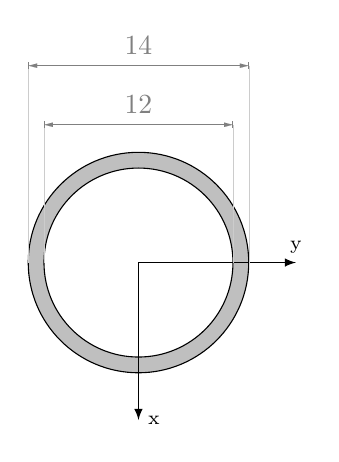
\begin{tikzpicture}
%linee guida
%\foreach \x in {0,1,...,15}
%   \draw [help lines] (\x,0) node [below,%
%          font=\footnotesize] {$\x$} -- (\x,15);
%\foreach \y in {0,1,...,15}
%   \draw [help lines] (0,\y) node [left,%
%          font=\footnotesize] {$\y$} -- (15,\y);

% InternalRadius, 0.012
% ExternalRadius, 0.014
\draw[fill=lightgray] (7.5,7.5) circle (14mm);
\draw[fill=white] (7.5,7.5) circle (12mm);
%reference system
\draw[-latex] (7.5,7.5)--(7.5,5.5)node[right]{\scriptsize x};
\draw[-latex] (7.5,7.5)--(9.5,7.5)node[above]{\scriptsize y};

%% quote track
 \dimline    [color=gray,
 			  label style={above=0.1ex},
                % line style={thick},
                %extension start style={gray,thin},
                %extension end style={gray,thin},
                extension start length=1.75cm,
                extension end length=1.75cm
                ]{(7.5-1.2,9.25)}{(7.5+1.2,9.25)}{$12$};
                
\dimline    [color=gray,
			 label style={above=0.1ex},
                % line style={thick},
                %extension start style={gray,thin},
                %extension end style={gray,thin},
                extension start length=2.5cm,
                extension end length=2.5cm
                ]{(7.5-1.4,10)}{(7.5+1.4,10)}{$14$};
\end{tikzpicture}}
\caption{Shaft's tubolar section}
\label{fig:SectCTube}
\end{figure}
To make rigid connections, elements of type: \textsc{mpc184}, with key option: $1$,used to block six degrees of freedom. Moreover, they have resistance properties equal to those of the extruded steel for the beam elements. 
Note that they were used without densities because the default section in \textsc{ansys} is equal to $1$ for default, this because they caused an overstimation in mass calculation and then in the derived natural frequencies of the modal analysis.
Finally, we consider the mass concentrated near the end of the queue representing the tail rotor block, this simplification is static represented by elements of the type: \textsc{mass21}, to which the following mass and inertia properties were assigned:
\begin{itemize}
\item concentrated mass: $30\,[kg];$
\item concentrated inertia:  $1\,[kg*m^2]$. 
\end{itemize}
The result is visible in fig. \ref{fig:Ansys1MeshShaft}

\begin{figure}[ht]
\centering
\subfloat[][\emph{side view}.]
   {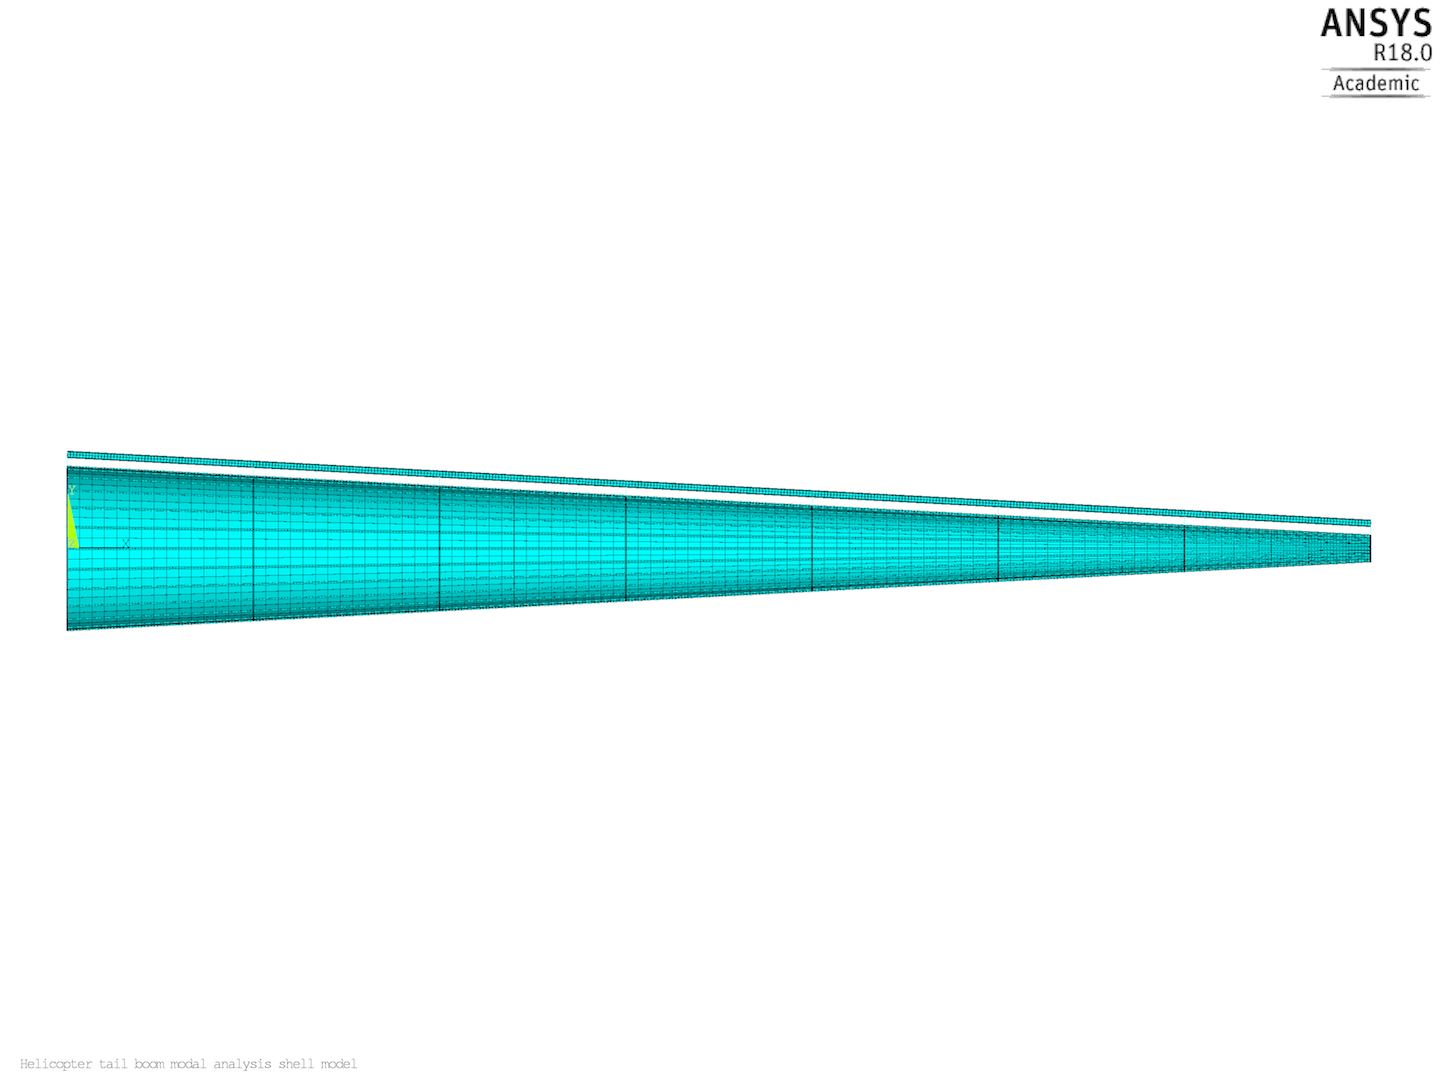
\includegraphics[width=.45\textwidth]{/ShellModelShaft/ShellmodelShaft001}} \quad
\subfloat[][\emph{isometric view}.]
   {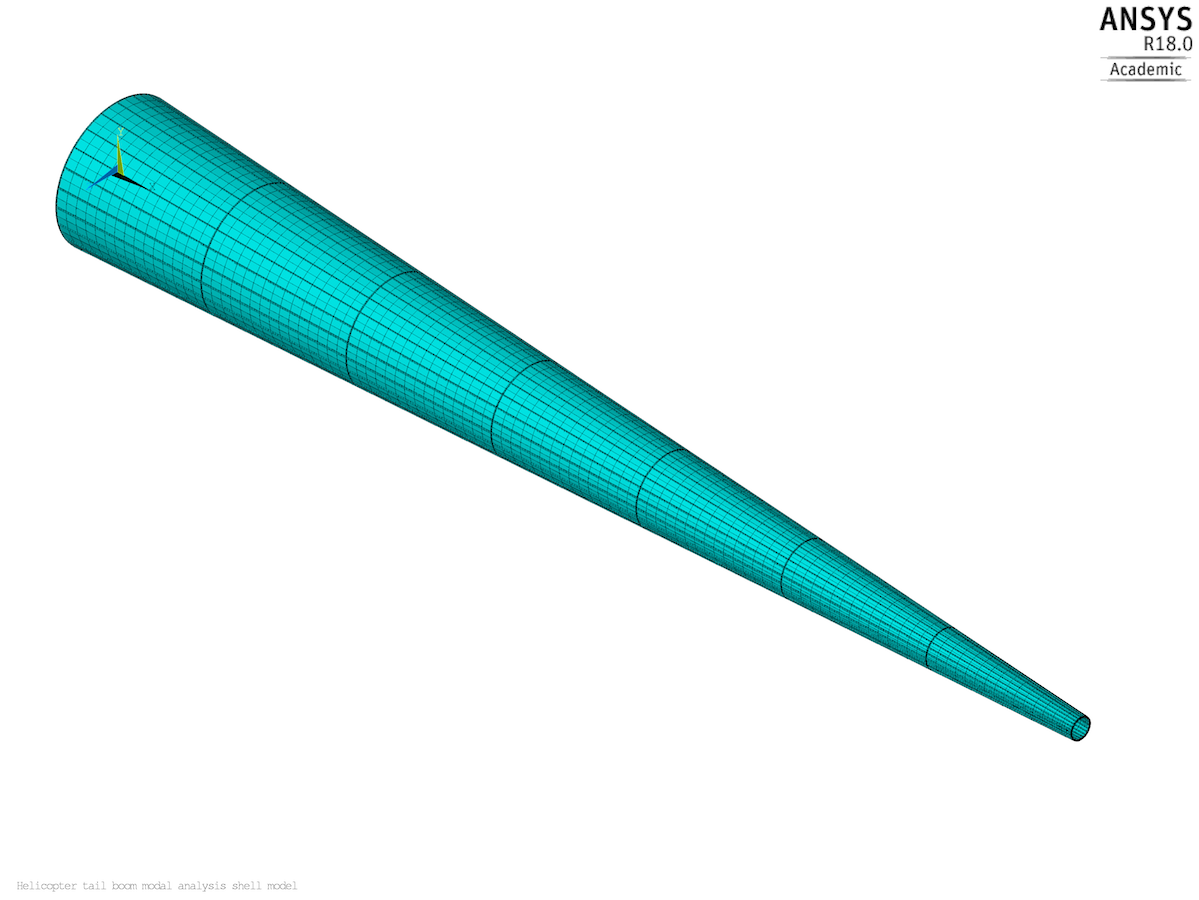
\includegraphics[width=.45\textwidth]{/ShellModelShaft/ShellmodelShaft002}}\\
\caption{Shell model with shaft}
\label{fig:Ansys1MeshShaft}
\end{figure}

\subsection{Simple model with lumped mass}
Starting with the simple model, in this case, the rigid rigid links are added as done to the model with the shaft, but in this case in the connecting terminal part are added the concave mass portions representing the distributed shaft weight. In fact, these are modeled with \textsc{mass21} element type and have the property of having the mass equal to a fraction of the shaft.
Also in this case consider the rotor block as near the tail as modeled in the previous case, the result is visible in Figure 2.
%% inserire immagini

\section{Preliminary analysis}
In the preliminary analysis we have investigated the deformations caused by the proper weight of the structure, in fact this is only subject to gravity acceleration, using an approximate value equal to $9.81\,[m/s^2]$.
Each model has been studied by making it a constraint with a cone at the base of the cone, so it is possible to make a parallelism with a cantilever beam.
In the following, table \ref{tab:RecapStressDeformation}, shows deflection and stress values while you can observe the effects of flexural tension distribution for structures and the effect due to the presence or not of the shaft, osservable in figures \ref{fig:ShellNodalSolu}--\ref{fig:ShellVonMises}.
\begin{table}[!ht]
\centering
\begin{tabular}{lcc}
\hline
Case				& Displacement 	& 	Stress\\
				& $[mm]$			&	$[MPa]$\\
\hline
Simple model		& value 			& 	value\\
With shaft		& value 			& 	value\\
Lumped mass		& value 			& 	value\\
\hline
\end{tabular}
\caption{Deformation values and stress of the models analyzed}
\label{tab:RecapStressDeformation}
\end{table}
\begin{figure}[ht]
\centering
\subfloat[][\emph{Simple model}.]
   {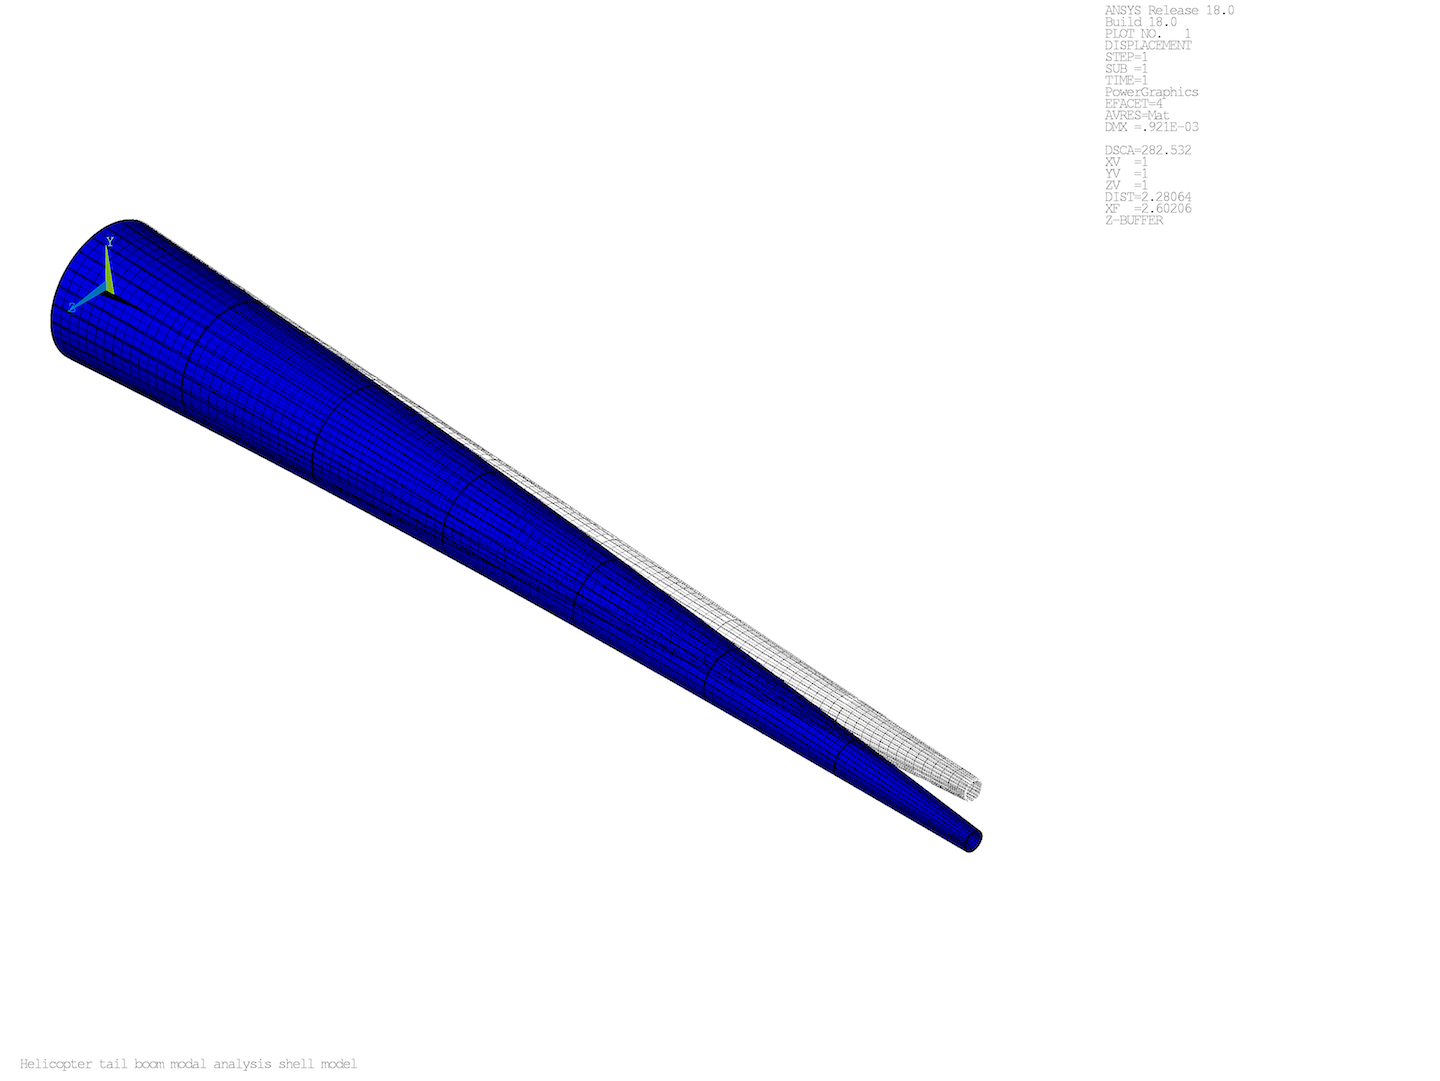
\includegraphics[width=.45\textwidth]{/ShellModel/Shellmodel003}} \quad
\subfloat[][\emph{Model with Shaft}.]
   {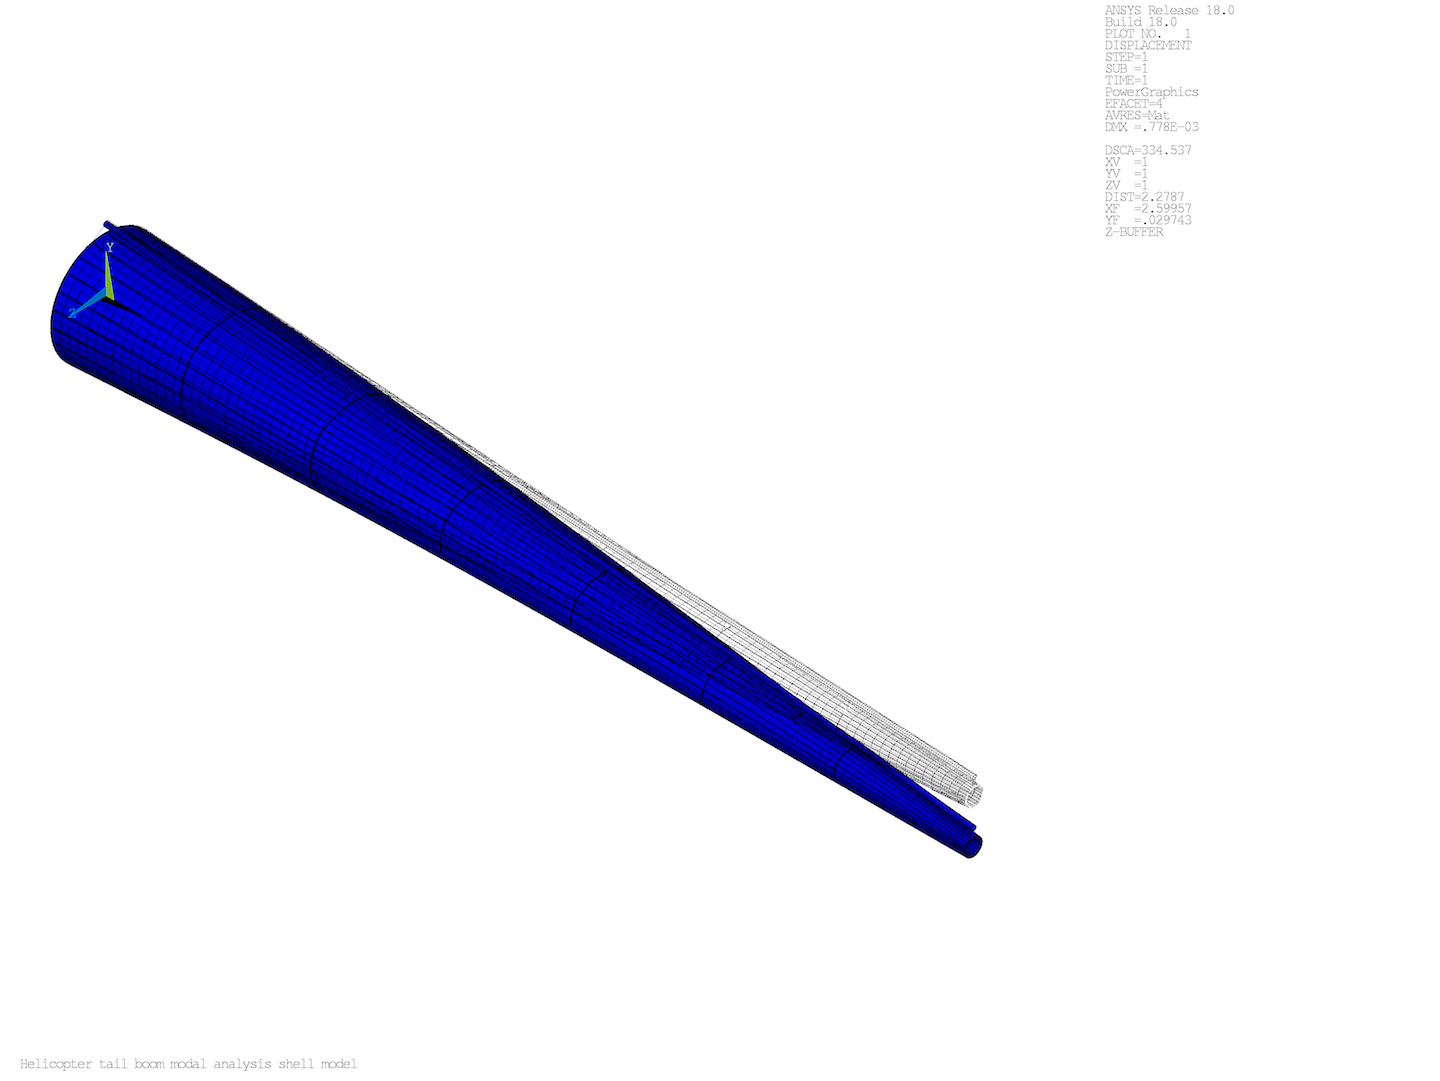
\includegraphics[width=.45\textwidth]{/ShellModelShaft/ShellmodelShaft004}} \\
   \caption{Maximum displacement}
   \label{fig:ShellDisplacement}
\end{figure}

\begin{figure}[ht]
\centering
\subfloat[][\emph{Simple model}.]
   {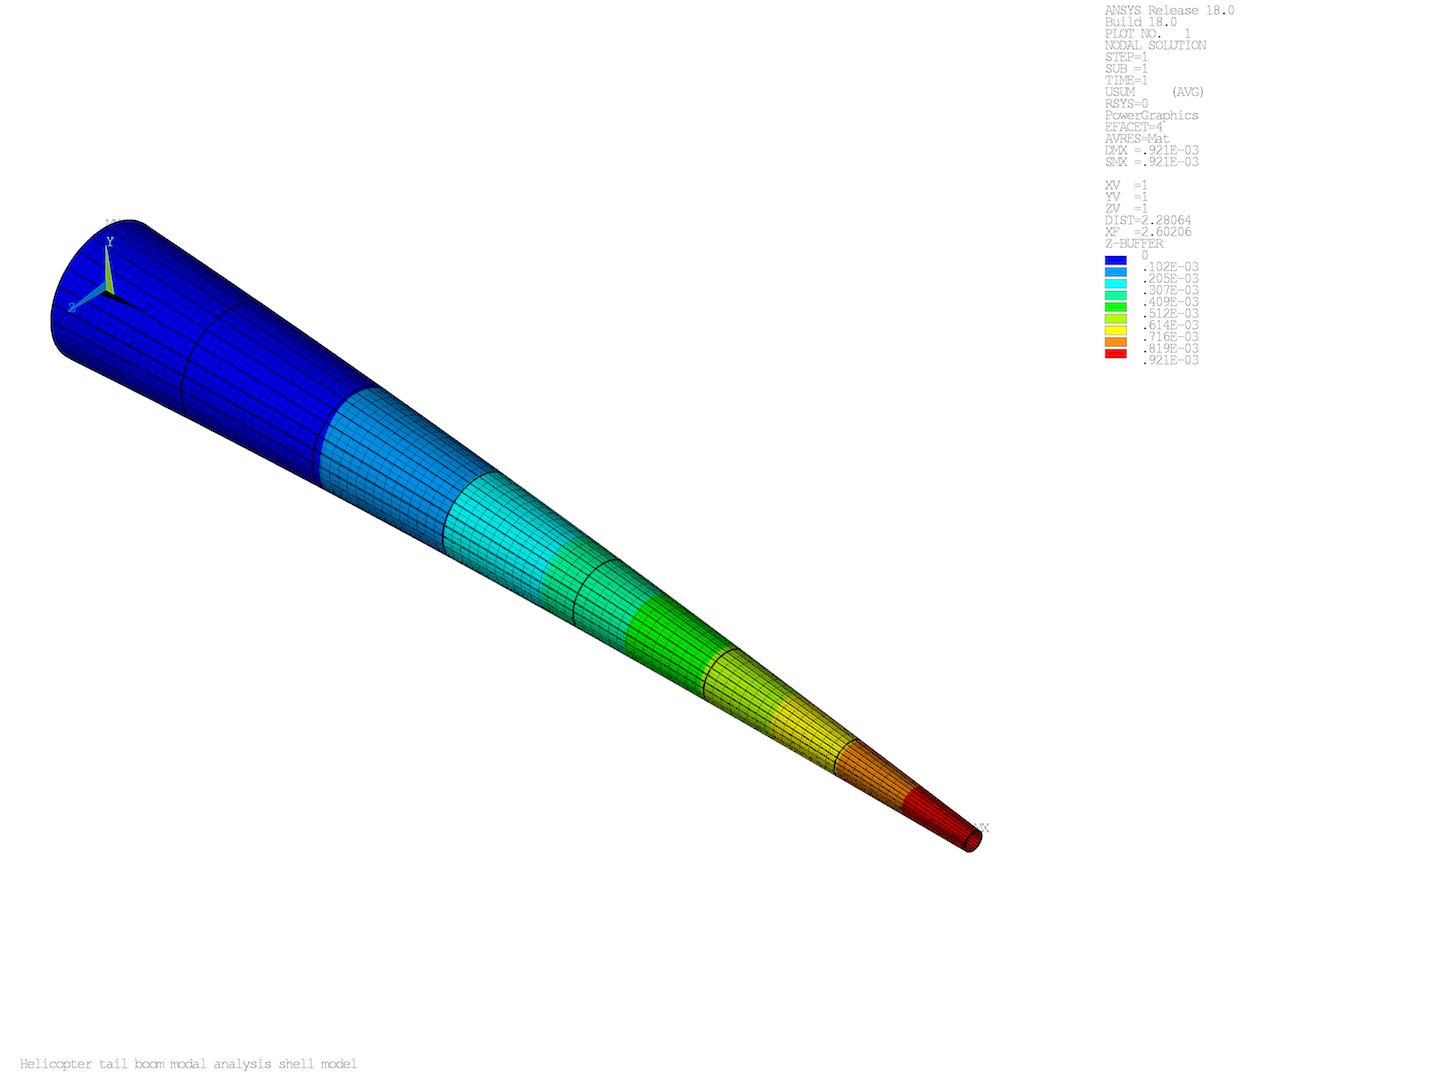
\includegraphics[width=.45\textwidth]{/ShellModel/Shellmodel004}} \quad
\subfloat[][\emph{Model with Shaft}.]
   {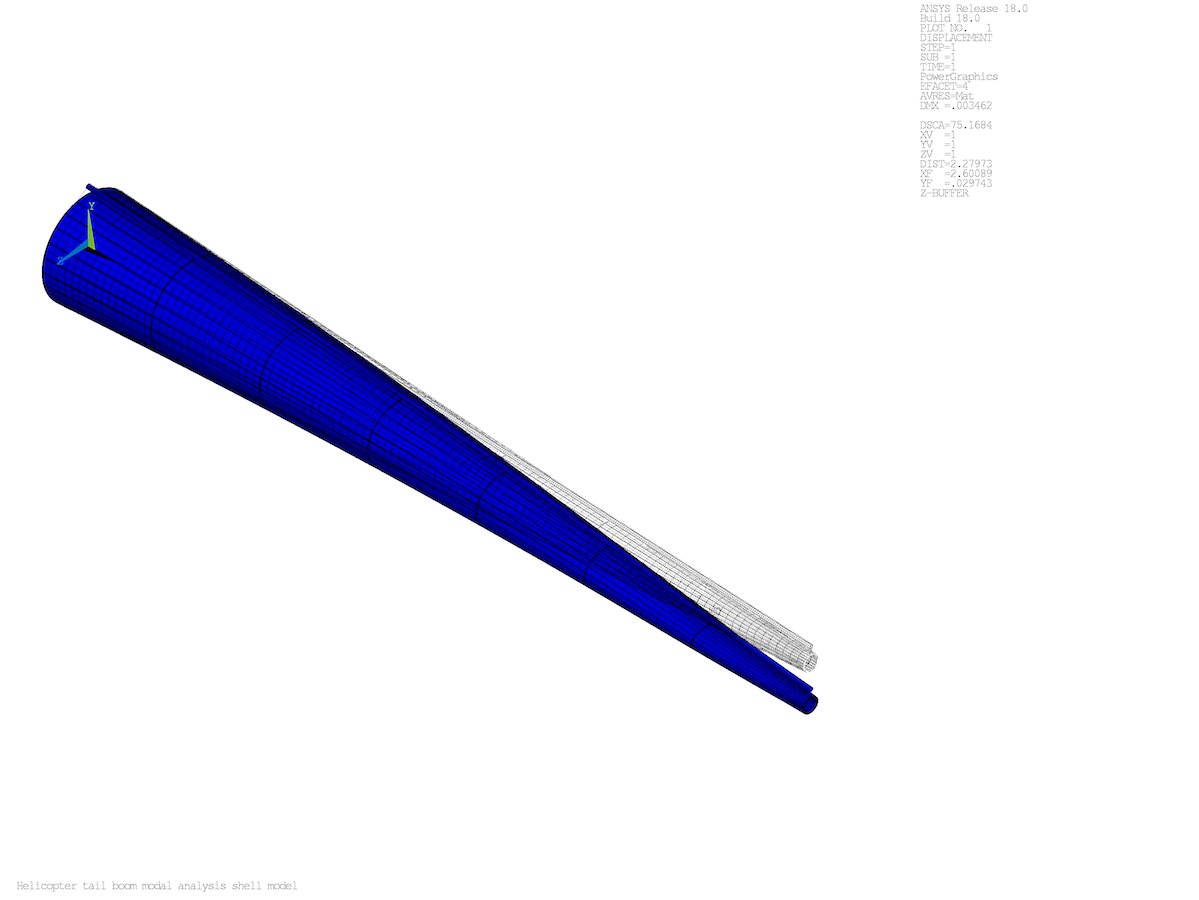
\includegraphics[width=.45\textwidth]{/ShellModelShaft/ShellmodelShaft005}}\\
\caption{Nosal soluiton}
\label{fig:ShellNodalSolu}
\end{figure}

\begin{figure}[ht]
\centering
\subfloat[][\emph{Simple model}.]
   {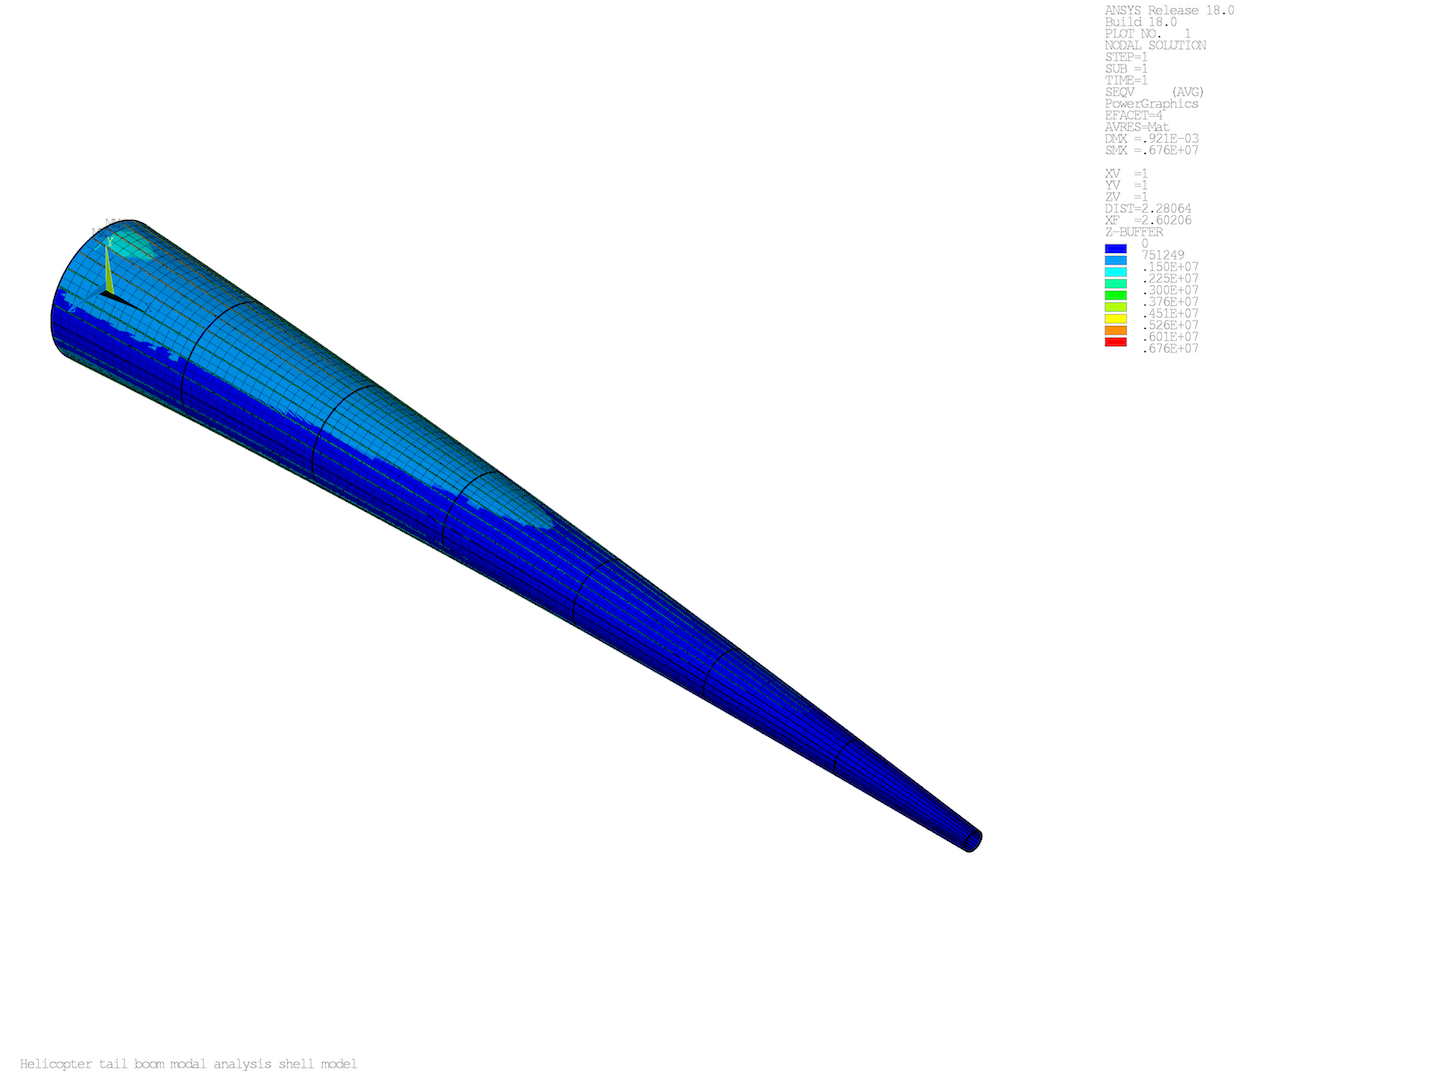
\includegraphics[width=.45\textwidth]{/ShellModel/Shellmodel005}} \quad
\subfloat[][\emph{Model with Shaft}.]
   {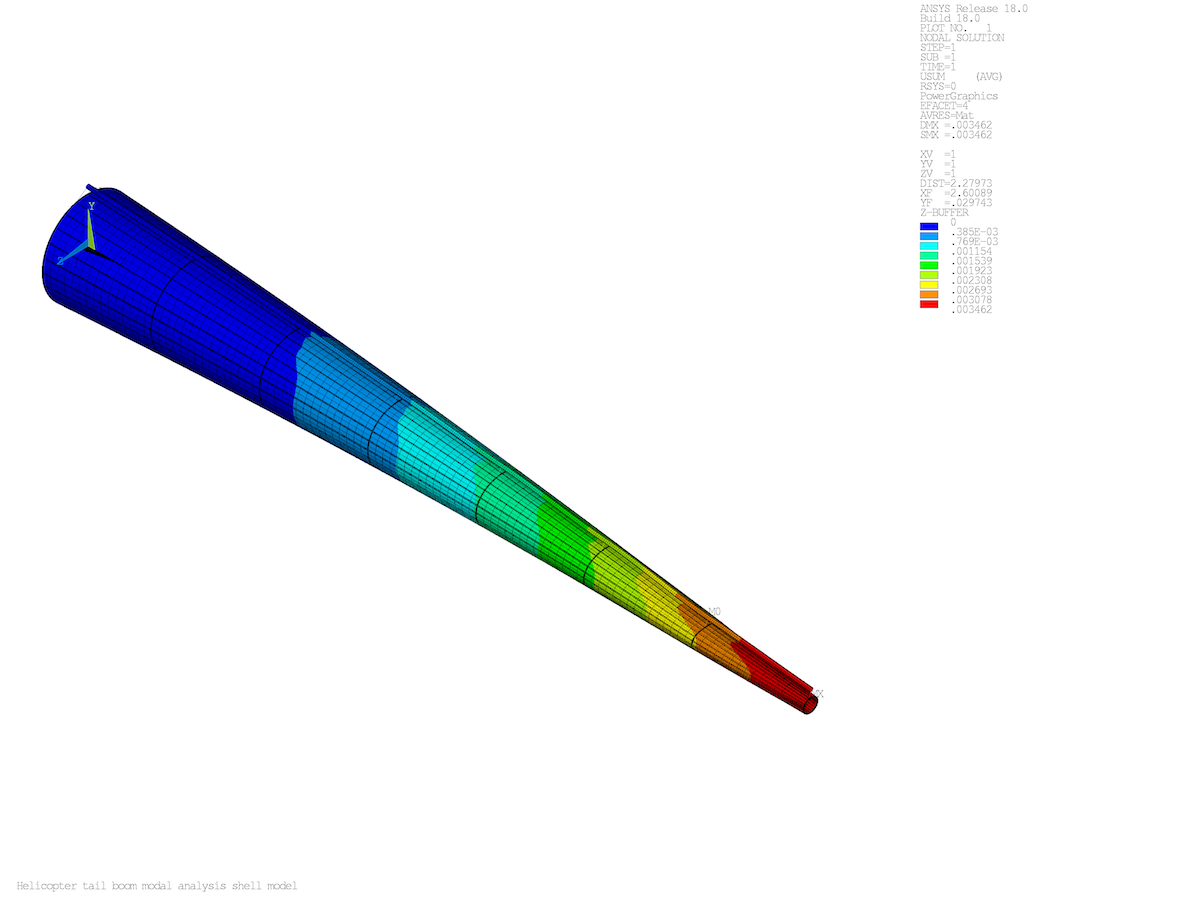
\includegraphics[width=.45\textwidth]{/ShellModelShaft/ShellmodelShaft006}}\\
\caption{Von Mises equivalent stress}
\label{fig:ShellVonMises}
\end{figure}

\section{Modal Analysis}
\begin{table}[h!]
\centering
\pgfplotstableset{
	% global config, for example in the preamble
	% these columns/<colname>/.style={<options>} things define a style
	% which applies to <colname> only.
    every head row/.style={before row=\hline,after row=\hline},
    every last row/.style={after row=\hline},
    display columns/0/.style={column name =Mode, int detect,column type=r},
    display columns/1/.style={column name =Frequence [Hz], column type=r,
	fixed,fixed zerofill,precision=5,set thousands separator={\,}},
    %other style option   
    }
    \pgfplotstabletypeset[col sep=space]{ModalFreq-ShellmodelShaftLumped.txt}
\caption{Estimated Data.}
\end{table}
	% Inserite qui gli altri capitoli:

	%%%%%%%%%%%%%%%%%%%%%%%%%%%%%%%%%%%%%%%%%%%%%%%%%%%%%%%%%%%

\chapter{Conclusioni}
\label{ref:Conclusioni}

Spero che la guida possa servirvi ragazzuoli!\\\\

\noindent Ringrazio di cuore Giordano Cardillo e Matteo Merola per avermi aiutato (e sopportato) a capire come funziona questo maledetto \LaTeX ! :P

Ringraziate Giordano anche per aver creato dei loghi vettoriali decenti da utilizzare :D (li trovate nella cartella delle immagini).\\\\\noindent 

\noindent Vi voglio bene <3 (tranne a Rosangela u.u)\\\\

\begin{flushright}
\textit{Guida scritta da Lorenzo Valente} \footnote{http://facebook.com/lorenzo.valente}
\end{flushright}
	\lstlistoflistings
	% === Bibliografia ====================================
	\newpage
	\bibliographystyle{IEEEtran}
	\bibliography{bibliografia-tesi.bib}
	\chapter{Listing}
\section*{Shell Model}
\listingautocaption[language=apdl-modified, label={lst:ShellModel}]
{ShellModel.txt}
\listingautocaption[language=apdl-modified, label={lst:ShellModelShaft}]{ShellModelShaft.txt}
\listingautocaption[language=apdl-modified, label={lst:ShellModelShaftLumped}]{ShellModelShaftLumped.txt}
\listingautocaption[language=apdl-modified, label={lst:ShellModelRotor}]{ShellModelRotor.txt}
\listingautocaption[language=apdl-modified, label={lst:ShellModeldiskRun}]{ShellModeldiskRun.txt}
\section*{Macro}
\listingautocaption[language=apdl-modified, label={lst:testperson}]{testperson.mac}
\listingautocaption[language=apdl-modified, label={lst:generateimages}]{generateimages.mac}
\listingautocaption[language=apdl-modified, label={lst:rotor}]{rotor.mac}
\listingautocaption[language=apdl-modified, label={lst:relativereferencesystem}]{relativereferencesystem.mac}
\listingautocaption[language=apdl-modified, label={lst:distancenode}]{distancenode.mac}
\listingautocaption[language=apdl-modified, label={lst:calcmass}]{calcmass.mac}
\listingautocaption[language=apdl-modified, label={lst:getextremeaxis}]{getextremeaxis.mac}
\end{document}
